\subsection{Node structure and impact on the size of the tree}

As stated in the previous report, the order of the data in the node has been changed in order to have it use the least possible place.

At the begining of the project each node used to have its board game stored as a Bitboard and the move that led to it. As some nodes had the same state (Bitboard), we tried to use an unordered\_map in order to group them and decrease the size of the tree. However due to the high number of nodes, each time we created one we had to check wether or not it was referenced. As the size of the map kept increasing, therefore the time . This leads to a big diminution of the number of simulations and therefore decrease the reliability of the results provided.

As the algorithm goes down through the search tree, the game can be retraced by playing the chosen moves on the a clone of the root board. That way, we saved the space used by each nodes board.

\noindent
Size of a board : $120$ octets\\
Size of a node with the board : $168$ octets\\
Size of a node without the board : $48$ octets

With the same number of nodes this represent a diminution of the tree size by $70\%$. Therefore while using the same space, the improved tree is $3,5$ times bigger.

\subsection{Tree structure : List vs Array}

In december, each node used to contain the list of its children. Theses were allocated at the creation of the list. Thus the costly memory allocation was done during the exploration.
In order to improve this matter, we created a list of \"available nodes\" where nodes were allocated in the memory but not used by the tree. On exploration, they were moved to the children list. Whereas on prunning they were put back in that \"available nodes\" list.

While the idea is interesting, the children are not stored in continuous regions. During the UCT selection, each node children is visited, thus we didn't take advantage of cache. This is the reason why, on the advice of Pascal Garcia we moved on an array structure. At the begining of the programm, a large array of Node is allocated, making provisions for the follow up demands. Each node only has to contain the pointer to its first children and the number of them, thus making sure that they are stored subsequently. On loading the first child, with the processor optimisations, the followup are also loaded resulting to a great increase of speed.

Moving to a simple List implementation without pre-allocation to the Array structure and optimized implementation resulted to an increase of the number of simulations by 700\%.

\subsection{Prunning : Defragmentation model vs buffer copy model}

Two way of prunning the tree has been thought of. The first one, as  explained in the previous report, uses two arrays \textit{buffer} and \textit{tree}. While the second one uses only one array \textit{tree}.

The first and simplest one had three steps : \\
- copy only the selected nodes to the \textit{buffer} \\
- clean the first array (\textit{tree}) \\
- copy back the \textit{buffer} to the \textit{tree}.

The second one is inspired on the defragmentation of a hard disk drive the idea is not to copy the elements to be keep but move them inside the array. It is done in two steps : \\
- mark the nodes to be deleted. \\
- move the nodes in order to compact the tree. \\

\begin{figure}[H] 
\centerline{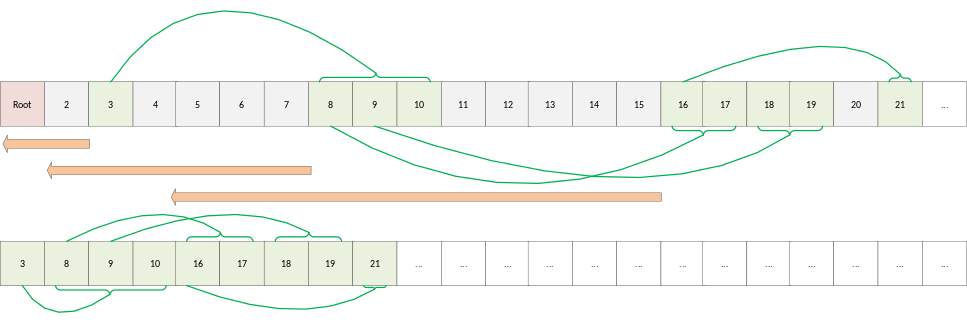
\includegraphics[width=\textwidth]{Optimisations/array.png}}
\caption{\label{fig:Defrag}\textit{defragmentation model, the nodes are compacted to the left.}}
\end{figure}

The aim of this method is to use the RAM for only one tree instead of having to use half of it due to the \textit{buffer}. That way the size of the tree is increased by 50\%.

However that second method requires many more updates than expected : 
each time a node is moved, it is required to change the pointer of its parent if it is the first node. It also require to update the parent pointer of its children. All this increase greatly the call in the memory. In order to solve such a problem, we used another array, \textit{index} which reference the adress of each node. On moving one, it is only required to change its reference while the parent and children point to that redirection.

While the benefits of such implementation is clear. On greater trees the time spend compacting grows too much in comparison to the first method. Due to such heavy drawback. That second method has been droped.

\subsection{Scalling on multicore machine}

A bench mode (\textit{-b} or \textit{--bench}) has been implemented in order to easily follow the evolution of the scaling through the subsequent iterations and improvements. We had access to rodrigue an old (2009) 24-core-server. It permited us to compare the number of simulations done by our algorithm through an increasing number of core (see the following figures).

\begin{figure}[H] 
\centerline{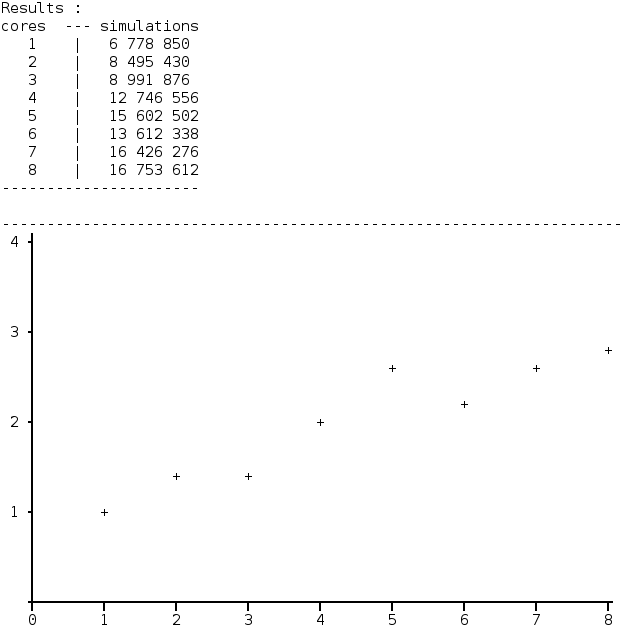
\includegraphics[width=0.8\textwidth]{Optimisations/bench_T1700.png}}
\caption{\label{fig:Defrag}\textit{Bench test on Dell Precision T1700 (4 physical cores, 8 logical cores)}}
\end{figure}

It is shown that the number of simulations scales not that well with the number of cores. We expected better results. However these figures are probably due to a poor implementation.
We could also notice on rodrigue that from 9 cores, the number of simulations stabilize. This might be caused by a possible the saturation of memory bus as a resulted of too many access from the processors and a possible recuring cache invalidation.

\begin{figure}[H] 
\centerline{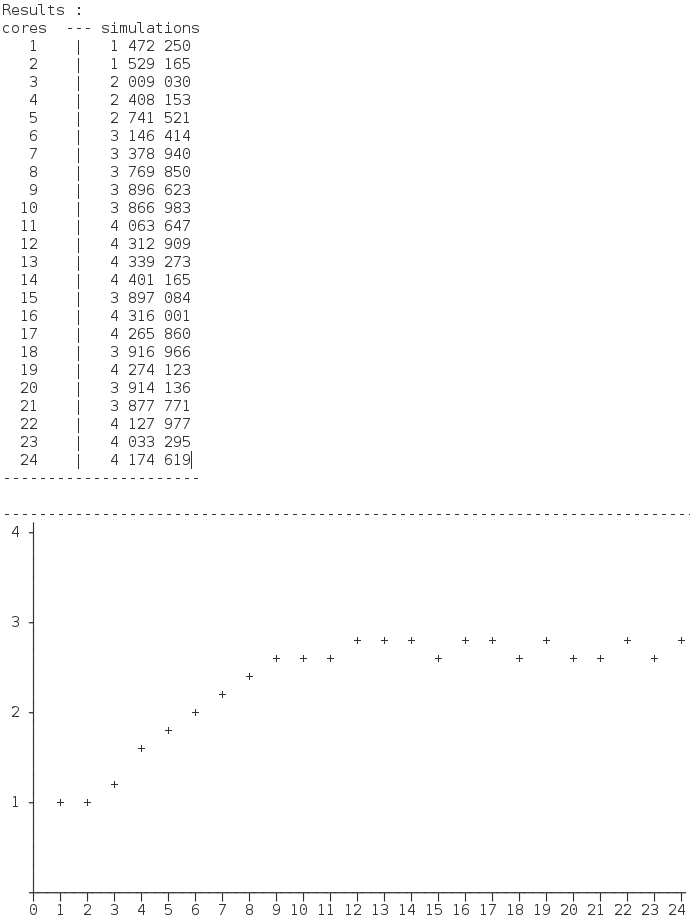
\includegraphics[width=\textwidth]{Optimisations/bench_rodrigue.png}}
\caption{\label{fig:Defrag}\textit{Bench test on rodrigue (24 physical cores, 24 logical cores)}}
\end{figure}


